\documentclass[a4paper,11pt]{article}

% fonts
\usepackage[p,osf]{cochineal}
\usepackage[scale=.95,type1]{cabin}
\usepackage[cochineal,bigdelims,cmintegrals,vvarbb]{newtxmath}
% fixed width font with 80 chars per listing line
\usepackage[scaled=.94]{newtxtt}
\usepackage[cal=boondoxo]{mathalfa}

% make the document take up more of the page
\usepackage[margin=1in]{geometry}

% no paragraph indent
\usepackage[parfill]{parskip}

% plotting mathematical functions (needs version request)
\usepackage{pgfplots}
\pgfplotsset{compat=1.15}

% \url function and clickable table of contents. no ugly red boxes though
\usepackage[hidelinks]{hyperref}

% maths symbols and other stuff (supersedes the ams* packages)
\usepackage{mathtools}
\usepackage{amssymb}

% more advanced handling of utf8 and fonts or something. apparently good to have
\usepackage[utf8]{inputenc}
\usepackage[T1]{fontenc}

% graphics, like eps files and stuff (supersedes graphics)
\usepackage{graphicx}

% used to horizontally align floats
\usepackage{subfig}

% used for figures
\usepackage{float}

% needed for colouring and stuff (xcolor supersedes color)
\usepackage{xcolor}

\definecolor{codegreen}{rgb}{ 0,0.6,0}

% listings of code
\usepackage{minted}
\setminted{breaklines,
           breakbytokenanywhere,
           linenos
}
\usemintedstyle{friendly}
% bigger line numbers
\renewcommand\theFancyVerbLine{\footnotesize\arabic{FancyVerbLine}}

% that can break across pages while being captioned figures
\usepackage{caption}
\newenvironment{longlisting}
{\addvspace{\baselineskip}\captionsetup{type=listing}}
{\addvspace{\baselineskip}}
% allow maths to break across pages
\allowdisplaybreaks

\begin{document}

\begin{center}
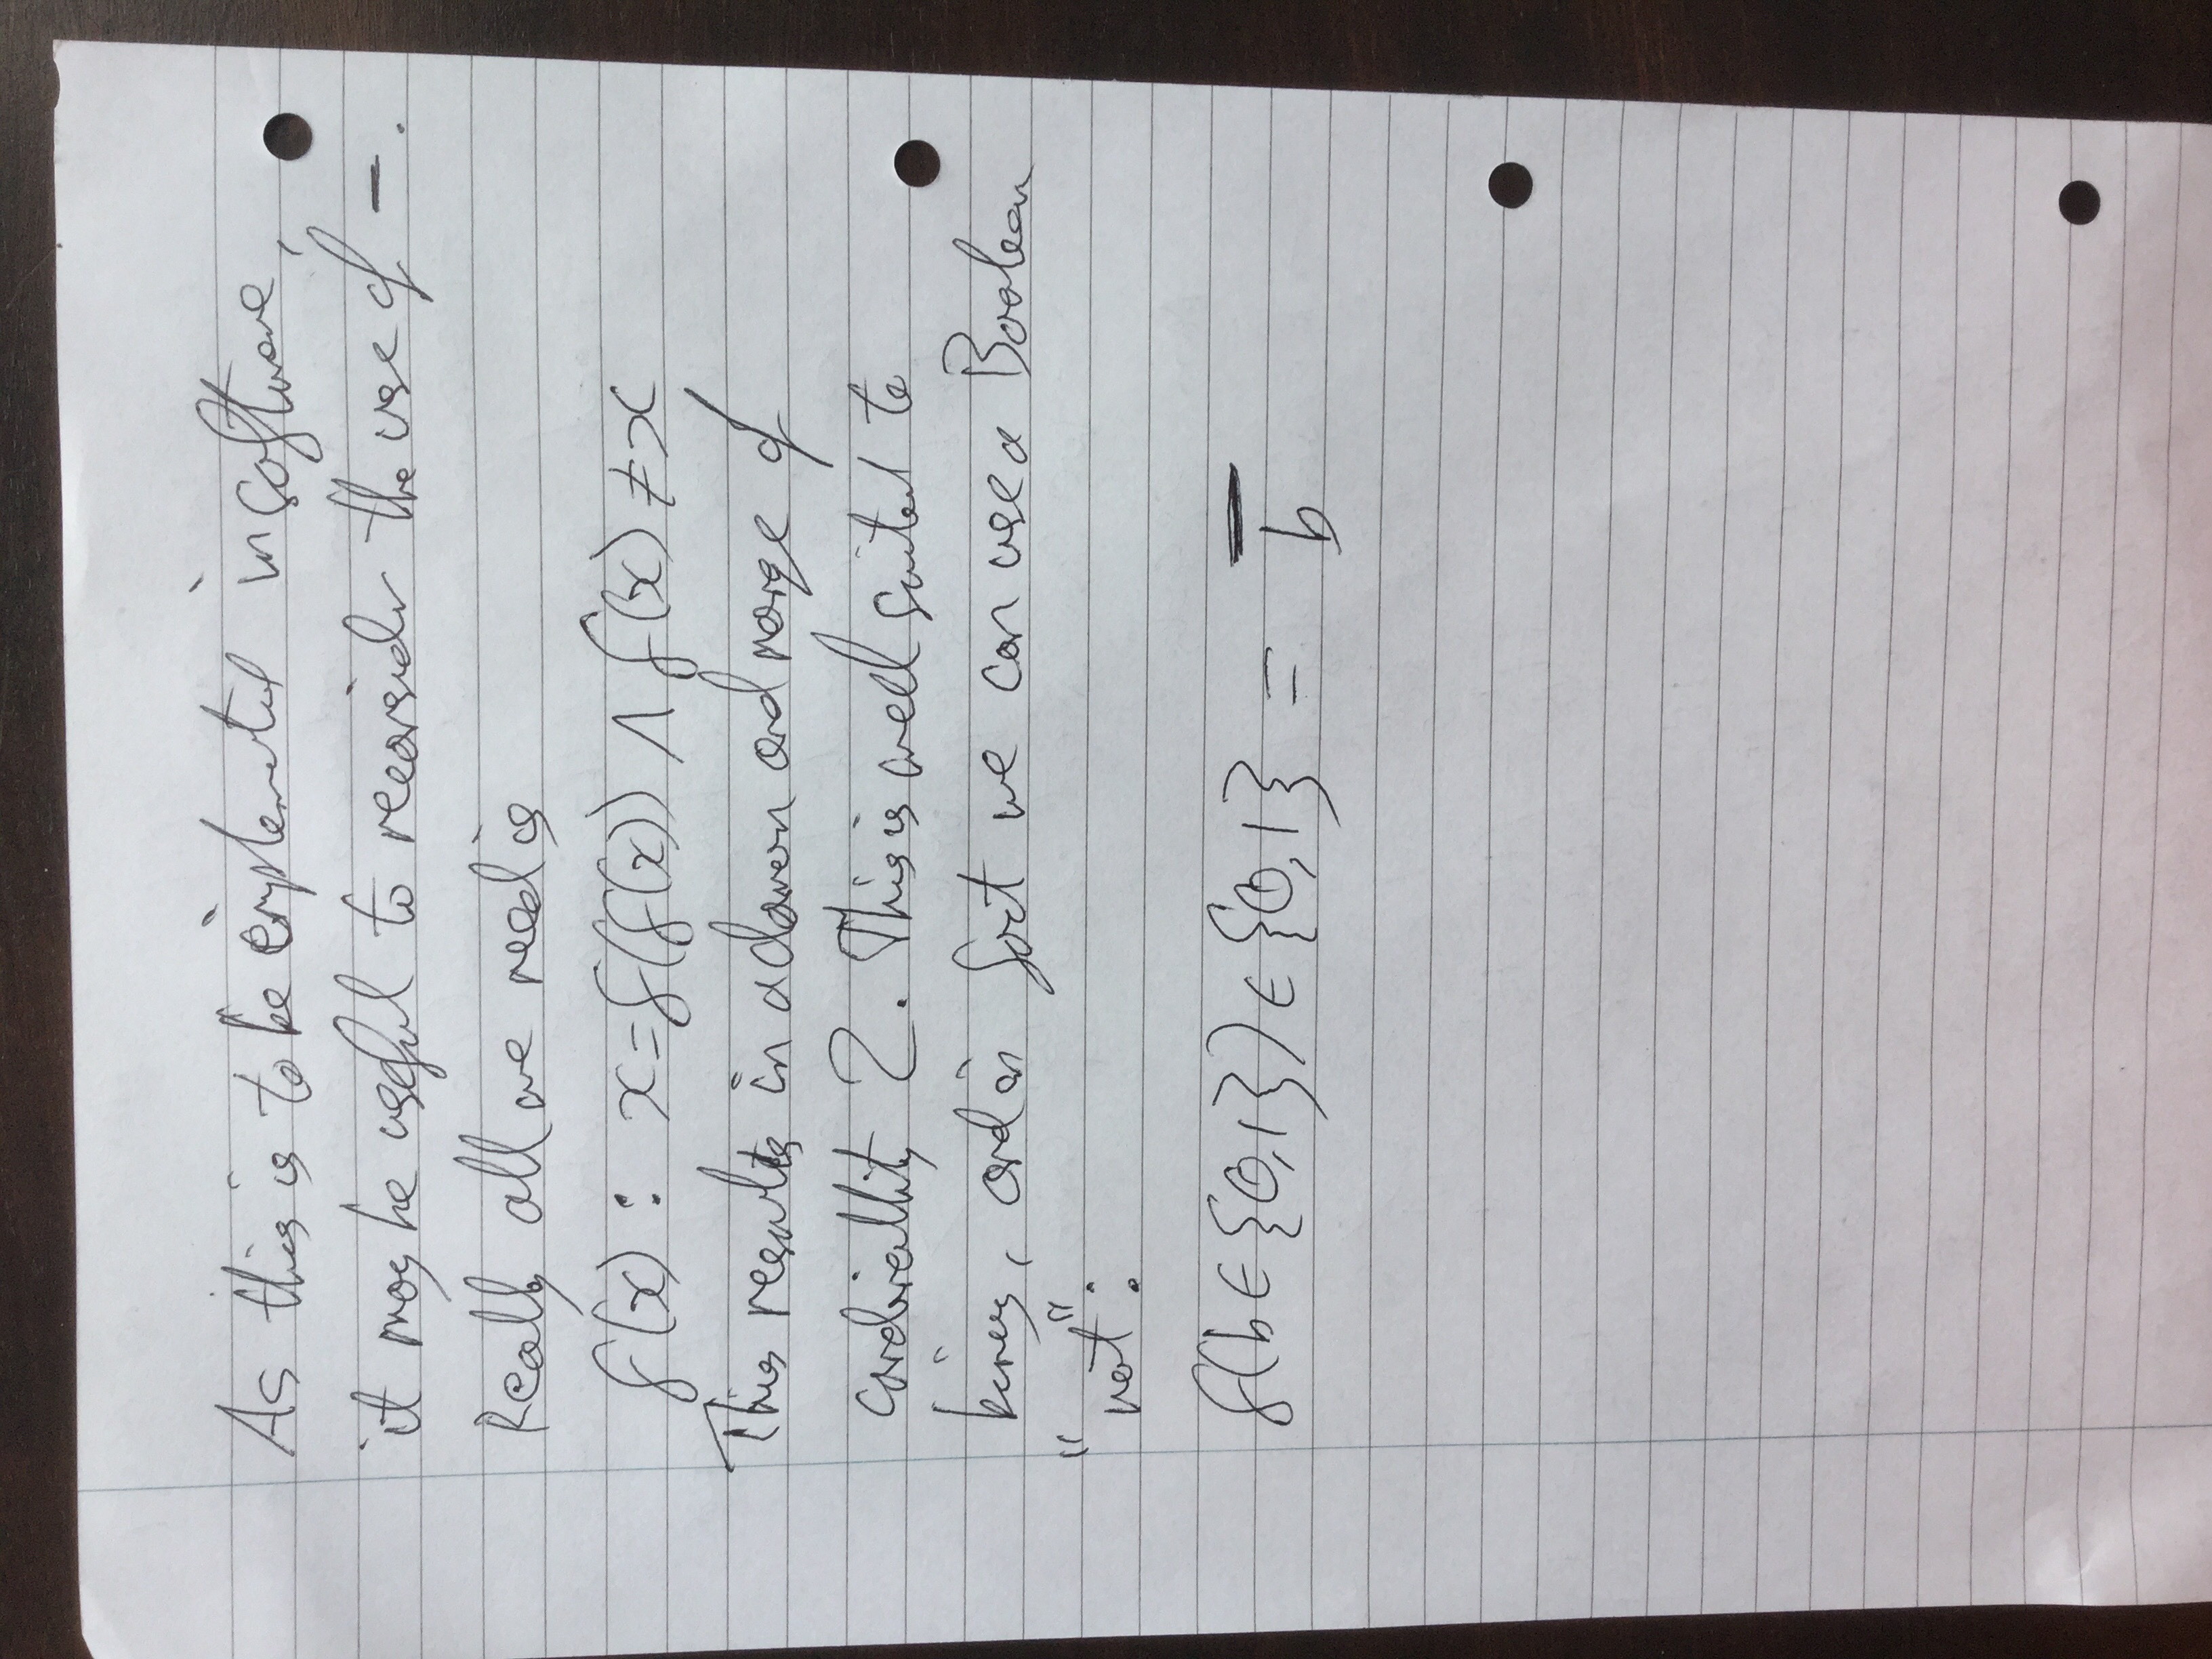
\includegraphics[height=\textheight]{../psfiles/hadamard_2.eps}
\end{center}
\newpage
\begin{center}

\includegraphics[height=\textheight]{../psfiles/hadamard_3.eps}
\end{center}
\newpage
\begin{center}

\includegraphics[height=\textheight]{../psfiles/hadamard_4.eps}
\end{center}
\newpage
\begin{center}
\includegraphics[height=\textheight]{../psfiles/hadamard_5.eps}
\end{center}

\end{document}
